\documentclass[sigconf]{acmart}

\AtBeginDocument{%
  \providecommand\BibTeX{{%
    \normalfont B\kern-0.5em{\scshape i\kern-0.25em b}\kern-0.8em\TeX}}}


\copyrightyear{2022}
\acmYear{2022}
\setcopyright{acmcopyright}
\acmDOI{}
\acmPrice{}
\acmISBN{}

%% These commands are for a PROCEEDINGS abstract or paper.
\acmConference[Parallel Programming@NYCU]{January 9,
  2022}{Hsinchu, Taiwan}


\begin{document}

%%
%% The "title" command has an optional parameter,
%% allowing the author to define a "short title" to be used in page headers.
\title{Game Tree Search on Gomoku}

%%
%% The "author" command and its associated commands are used to define
%% the authors and their affiliations.
%% Of note is the shared affiliation of the first two authors, and the
%% "authornote" and "authornotemark" commands
%% used to denote shared contribution to the research.
\author{Tsung-Fang, Chen}
\affiliation{
 \institution{NYCU}
 \state{0816153}
 \country{Taiwan}
}

\author{Tseng, Yang}
\affiliation{
  \institution{NYCU}
  \state{310554039}
  \country{Taiwan}
}



\begin{abstract}

We implemented Minmax and MCTS algorithms, parallelized both algorithms, and modified gomoku GUI interface to simulate how AI will react against humans.

Upon that, we also allowed users to dynamically tune the maximum depth, time, and threads for each step of calculation. By doing so, we can have a direct feeling of how each parameter will affect the response time and strength for the AI.

From the experiments below, we can see that after parallelization, we successfully gave the Minimax algorithm an average of 30\% speed up per thread, and 70\% speed up per thread on the MCTS algorithm.

\end{abstract}

\keywords{}
\maketitle






\section{Introduction}

People’s ambition is human nature. Everyone does not want to lose even in a small game. So many scientists use computers as their simulator of decision for choosing the game’s next move to maximize the winning chance. 

Currently, aside from the DNN approach (ex. GomokuNet),  Minmax and MCTS still play a critical role in gomoku AIs. However, both of the algorithms usually take a lot of time to compute, the linearity increase on strength results in an exponential increase for calculation time. Calculation taking too long will cause players to lose patience, while easy-beaten AIs will be of no use for amateaur or even professional players.

There are two ways to achieve our goal: Build an AI with certain strength and acceptable calculation time. The first solution is to invent a more efficient algorithm, which is not in our consideration for the certain final project. The second solution is to speed up the current method for gomoku AI, where parallelization comes in handy. We would like to utilize what we learn in this class to speed up the calculation.







\section{Proposed Solution}

We introduced two algorithms to solve this problem, Min-Max (Neg-Max) and MCTS. The board would be input as our program, and other parameters as well. The program would run the specific algorithm with the parameter we set. Output the json file to the frontend and show the movement to the user.


% ~~~~~~~~~~~~~~~~~~~~~ 
\subsection{Min-Max Tree}

The Min-Max tree could be modified to the Nega-Max tree. This could highly reduce the implementation detail and do exactly the same thing. For parallelism, we introduce the following thinking and implementation:
 
\begin{itemize}
\item {\verb|Board Evaluation|}
\item {\verb|Parallel Children|}
\item {\verb|Parallel with alpha-beta pruning |}
\end{itemize}

{\bfseries Board Evaluation:}
In Min-Max tree search, we have to evaluate each board’s score on the computer to determine if the movement is good or not. Board’s score comes from a few nodes in a row, blocking or not, and one move to win … etc. We divide the board by the number of threads we use. Each thread calculates the score in different regions, and sum up at the end. By experiment, the speed up is not obvious. The reason we speculate is because the board size is small. So we didn’t apply this parallelization in the final code.

{\bfseries Parallel Children:}
At the beginning of Min-Max tree search, the first layer (all the possible moves) enqueue into a queue. Nodes are equally distributed to each thread. Thread simulates the board for two user’s moves and expands to the depth we set (maxDepth).  

{\bfseries Parallel with alpha-beta pruning:}
Alpha beta pruning could speed up the min-max tree search. Did not expand for the node (movement) which is not possible because the value is not better than the previous already expanded node. Each thread would hold their own copy of alpha and beta value, and update(push or pull) the global alpha beta if found that it is better or old value. There would be some nodes which cut off very early which cause that each thread work load is not balanced. We introduce another approach, dynamically allocating the node to thread. If the thread ends early, it would ask for another node in the queue to expand. This would make the thread work almost equally. Try to maximize the threads and CPU usages.

{\bfseries Branching Factor:}
Branching factor is not a way for parallel programming. It’s a way to speed up the program via reducing the nodes for searching and expanding. When searching trees go deeper, the possibility of actually going to this board is getting smaller. So in the Min-Max algorithm, there is no need to evaluate the whole possibility of all possible moves. When the algorithm searches for the possible move in depth = 4 or deeper, it would only choose for at most 8 nodes with best board evaluation score to expand. But this would highly decrease the number of nodes, this makes the parallelism not visible. 


\subsection{Monte-Carlo Tree}

MCTS consists of four strategic phases, repeated as long as there is time left. The phases are as follows. (1) selection (2) expansion (3) simulation (4) backpropagation. In the selection step, the tree is traversed from the root node until it selects a leaf node L that is not added to the tree yet. Then, the expansion step is called to add the leaf node L to the tree. In the simulation step, the program plays random moves in a self-play mode until the end of the game is reached. In the backpropagation step propagates the result R of such a “simulated” game through the tree. By repeating the four phases, MCTS can evaluate moves well.

\begin{itemize}
\item {\verb|Leaf parallelization|}
\item {\verb|Root parallelization|}
\end{itemize}

{\bfseries Leaf parallelization:}
Leaf parallelization is one of the easiest ways to parallelize MCTS. To formulate it in machine-dependent terms, only one thread traverses the tree and adds one or more nodes to the tree when a leaf node is reached. Next, starting from the leaf node, independent simulated games are played for each simulated game propagated backwards through the tree by one single thread. 
There is a problem in leaf parallelization. The time required for a simulated game is highly unpredictable. Playing n games using n different threads take more time on average than playing one single game using one thread, since the program needs to wait for the longest simulated game. 

{\bfseries Root parallelization:}
The root parallelization works as follows. It consists of building multiple MCTS trees in parallel, with one thread per tree. Similar to leaf parallelization, the threads don’t share information when the separate MCTS trees are merged with their corresponding clones. For each group of clones, the scores of all games played are added. The best move is selected based on this grand total. This parallelization method only requires a minimal amount of communication between threads.



\section{Experimental Methodology}

We did five experiments in total. In each experiment, we used the same board and same depth for Min-Max search or the same time limit for MCTS algorithm.

For the fixed maximum depth in min-max tree search with or without alpha beta pruning, we focus on the runtime to search for the whole min max search tree. 

We have to set a maximum computation time for the MCTS algorithm. So we could not estimate the parallelism on run time. We determine the parallelism via the number of nodes searched in a fixed time. 

The testing environment is on Ubuntu 20.04.3 LTS (GNU/Linux x86\_64) running on Intel(R) Xeon(R) CPU E5-2690. 



\section{Experimental Results}


{\bfseries Experiment 1:}
With no alpha beta pruning, the program has to choose the best movement by evaluating the whole tree with the highest board evaluation score. We could see that the runtime becomes smaller as we use more threads in total. We confirm the number of nodes visited, moves evaluated, movement, and corresponding score all remains the same in case of malfunctioning. 

\text{Parameters}
\begin{itemize}
\item {\verb|Min-Max Algorithm|}
\item {\verb|No Alpha-Beta Pruning|}
\item {\verb|No Branch Factor|}
\item {\verb|Maximum depth = 4|}
\item {\verb|Nodes = 308394|}
\item {\verb|Evaluation count = 47258320|}
\end{itemize}
\begin{center}
  \label{tab:commands}
  \begin{tabular}{c c c c c}
    \toprule
    Thread(s)& Run Time(s) & Speed Up & Efficiency & Nodes count\\
    \midrule
    1 & 22.800 & 1.00 & 1.00 & 308394\\
    2 & 14.000 & 1.63 & 0.81 & 308394\\
    3 & 10.489 & 2.17 & 0.72 & 308394\\
    4 &  8.806 & 2.59 & 0.65 & 308394\\
    5 &  7.898 & 2.89 & 0.58 & 308394\\
    6 &  7.214 & 3.16 & 0.53 & 308394\\
    7 &  6.682 & 3.41 & 0.49 & 308394\\
    8 &  6.469 & 3.52 & 0.44 & 308394\\
    \bottomrule
  \end{tabular}
\end{center}
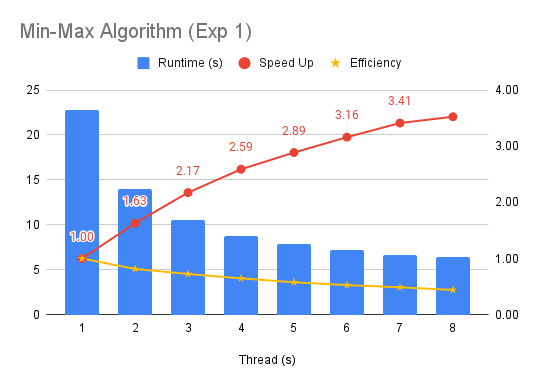
\includegraphics[scale=0.40]{images/exp1.png}



{\bfseries Experiment 2:}
As we enabled alpha beta pruning, the number of nodes significantly reduced from 308394 to 75211 on the same maximum depth. The runtime became too small for us to observe and compare the result of parallelism for multi threads. We confirm the number of nodes visited, moves evaluated, movement, and corresponding score all remains the same in case of malfunctioning. 
\text{Parameters}
\begin{itemize}
\item {\verb|Min-Max Algorithm|}
\item {\verb|Alpha-Beta Pruning|}
\item {\verb|No Branch Factor|}
\item {\verb|Queue Apply|}
\item {\verb|Maximum depth = 4|}
\item {\verb|Nodes = 75211|}
\item {\verb|Evaluation count = 12479778|}
\end{itemize}
\begin{center}
  \label{tab:commands}
  \begin{tabular}{c c c c c}
    \toprule
    Thread(s)& Run Time(s) & Speed Up & Efficiency & Nodes count\\
    \midrule
    1 & 4.183 & 1.00 & 1.00 & 75211\\
    2 & 2.560 & 1.63 & 0.82 & 75211\\
    3 & 2.042 & 2.05 & 0.68 & 75211\\
    4 & 1.574 & 2.66 & 0.66 & 75211\\
    5 & 1.395 & 3.00 & 0.60 & 75211\\
    6 & 1.304 & 3.21 & 0.53 & 75211\\
    7 & 1.228 & 3.41 & 0.49 & 75211\\
    8 & 1.237 & 3.38 & 0.42 & 75211\\
    \bottomrule
  \end{tabular}
\end{center}
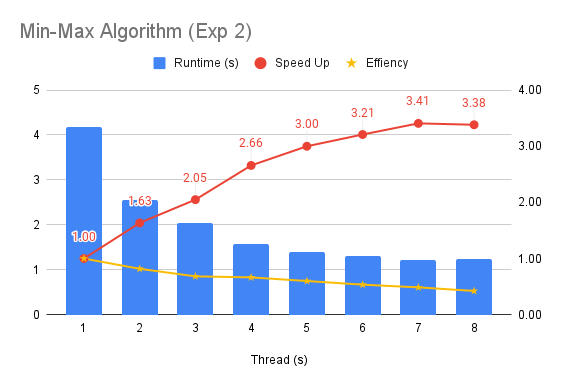
\includegraphics[scale=0.40]{images/exp2.png}


{\bfseries Experiment 3:}
Same constraint as experiment 2, except increasing the maximum depth to 5, making the number of nodes to 520681. From this experiment we could see that as the threads increase, the runtime decreases as we expected.  But the efficiency decreases slowly when threads increase. This situation was also in our expectation because more context switching leads to lower efficiency.

\text{Parameters}
\begin{itemize}
\item {\verb|Min-Max Algorithm|}
\item {\verb|Alpha-Beta Pruning|}
\item {\verb|No Branch Factor|}
\item {\verb|Queue Apply|}
\item {\verb|Maximum depth = 5|}
\item {\verb|Nodes = 520861|}
\item {\verb|Evaluation count = 90618342|}
\end{itemize}
\begin{center}
  \label{tab:commands}
  \begin{tabular}{c c c c c}
    \toprule
    Thread(s)& Run Time(s) & Speed Up & Efficiency & Nodes count\\
    \midrule
    1 & 30.644 & 1.00 & 1.00 & 520861\\
    2 & 18.738 & 1.64 & 0.82 & 520861\\
    3 & 14.112 & 2.17 & 0.72 & 520861\\
    4 & 11.778 & 2.60 & 0.65 & 520861\\
    5 & 10.774 & 2.84 & 0.57 & 520861\\
    6 & 9.574  & 3.20 & 0.53 & 520861\\
    7 & 8.907  & 3.44 & 0.49 & 520861\\
    8 & 9.032  & 3.39 & 0.42 & 520861\\
    \bottomrule
  \end{tabular}
\end{center}
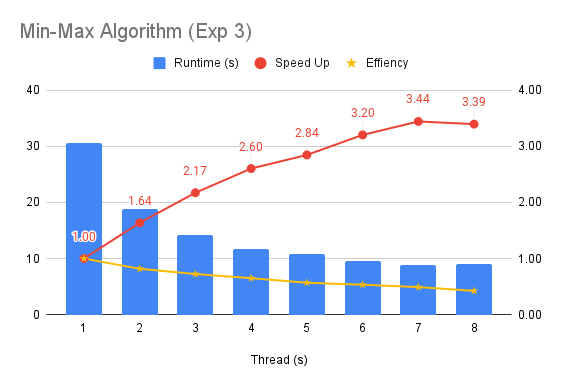
\includegraphics[scale=0.40]{images/exp3.png}



{\bfseries Experiment 4:}
When we added the branching factor to our algorithm, the number of nodes was only 20691 for maximum depth = 8. The runtime is too small so we could not easily observe the result of parallelism for multi threads.

\text{Parameters}
\begin{itemize}
\item {\verb|Min-Max Algorithm|}
\item {\verb|Alpha-Beta Pruning|}
\item {\verb|Branch Factor|}
\item {\verb|Maximum depth = 8|}
\item {\verb|Nodes = 20691|}
\item {\verb|Evaluation count = 280308|}
\end{itemize}
\begin{center}
  \label{tab:commands}
  \begin{tabular}{c c c c c}
    \toprule
    Thread(s)& Run Time(s) & Speed Up & Efficiency & Nodes count\\
    \midrule
    1 & 1.040 & 1.00 & 1.00 & 20691\\
    2 & 0.817 & 1.27 & 0.64 & 20691\\
    3 & 0.706 & 1.47 & 0.49 & 20691\\
    4 & 0.682 & 1.52 & 0.38 & 20691\\
    5 & 0.662 & 1.57 & 0.31 & 20691\\
    6 & 0.685 & 1.52 & 0.25 & 20691\\
    7 & 0.686 & 1.52 & 0.22 & 20691\\
    8 & 0.661 & 1.57 & 0.20 & 20691\\
    \bottomrule
  \end{tabular}
\end{center}
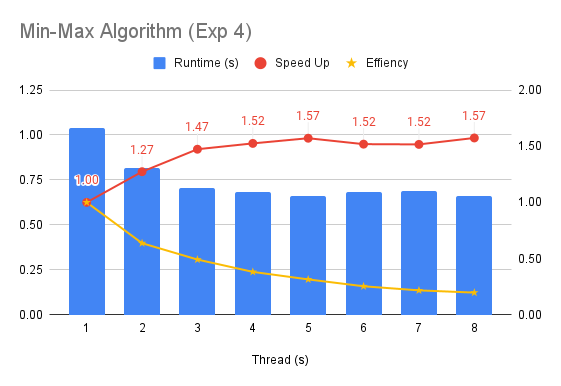
\includegraphics[scale=0.40]{images/exp4.png}




{\bfseries Experiment 5:}
MCTS algorithm could not consider runtime as the comparison factor for parallelism, because the MCTS takes it as the parameter and evaluates as many nodes in the limited time. Instead, we compare the efficiency of parallelism by counting the created nodes. When using multiple threads, there would be more nodes evaluated. We determined the efficiency of multi threads via the number of nodes visited in the algorithm. The results show that it’s up to 70\% speed up.

\text{Parameters}
\begin{itemize}
\item {\verb|MCTS Algorithm|}
\item {\verb|Leaf parallelization|}
\item {\verb|Root parallelization|}
\item {\verb|Maximum time = 5 seconds|}
\end{itemize}
\begin{center}
  \label{tab:commands}
  \begin{tabular}{c c c c}
    \toprule
    Thread(s)& Visit Count & Speed Up & Efficiency\\
    \midrule
     1 &  567736 & 1.00 & 1.00\\
     2 & 1092766 & 1.92 & 0.96\\
     3 & 1525638 & 2.69 & 0.90\\
     4 & 1945536 & 3.43 & 0.86\\
     5 & 2428195 & 4.28 & 0.86\\
     6 & 2863542 & 5.04 & 0.84\\
     7 & 3272241 & 5.76 & 0.82\\
     8 & 3732536 & 6.57 & 0.82\\
    16 & 4564848 & 8.04 & 0.50\\
    \bottomrule
  \end{tabular}
\end{center}
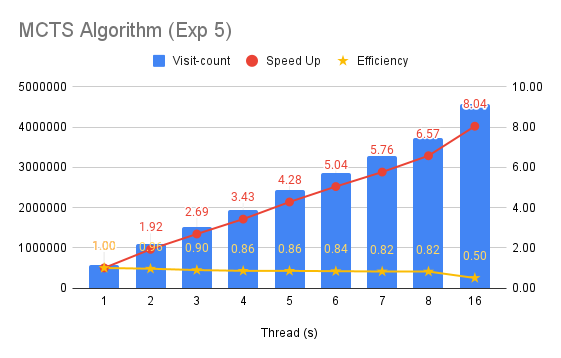
\includegraphics[scale=0.40]{images/exp5.png}



\section{Related work}
The first Monte-Carlo program is GOBBLE. It uses simulated annealing on a list of moves. The list is sorted by the mean score of the games where the move has been played. Moves in the list are switched with their neighbor with a probability dependent on the temperature. GOBBLE-like programs have a good global sense but lack tactical knowledge.

Another very effective way to combine search with Monte-Carlo has been found by R´emi Coulom with his program CRAZY STONE. It consists in adding a leaf to the tree for each simulation. The choice of the move to develop in the tree depends on the comparison of the results of the previous simulations that went through this node, and of the results of the simulations that went through its sibling nodes.







\section{Conclusions}
In the final project, we discussed the use of leaf parallelization and root parallelization for parallelizing MCTS and MiniMax with Alpha-Beta pruning. In the MCTS part, the speedup of the leaf and root parallelization is significant, and almost close to ideal conditions in small-scale threads. There is 70\% speedup per thread in MCTS parallelization on average , meaning that the parallelization for MCTS is efficient and suitable. In contrast, there are too many serial parts in MiniMax and Alpha-Beta pruning, so the efficiency for parallelizing MiniMax with Alpha-Beta pruning becomes lower with only 30\% speedup per thread on average.






\section{References}

\begin{itemize}
\item{\verb||}Produces colored hyperlinks.T. Cazenave and N. Jouandeau. On the parallelization of UCT. In H.J. van den Herik, J.W.H.M. Uiterwijk, M.H.M. Winands, and M.P.D. Schadd, editors, Proceedings of the Computer Games Workshop 2007 (CGW 2007), pages 93–101. Universiteit Maastricht, Maastricht, The Netherlands, 2007
\item{\verb||}G. Chaslot, M. Winands, and H. Herik. Parallel monte-carlo tree search. In Proceedings of the 6th international conference on Computers and Games, page 71. Springer-Verlag, 2008
D.E. Knuth and R.W. Moore. An analysis of alpha-beta pruning. Artificial Intelligence, 6(4):293–326, 1975
\item{\verb||}L. Kocsis and C. Szepesv´ari. Bandit Based Monte-Carlo Planning. In J. F¨urnkranz, T. Scheffer, and M. Spiliopoulou, editors, Machine Learning: ECML 2006, volume 4212 of Lecture Notes in Artificial Intelligence, pages 282–293, 2006
\item{\verb||}R. Coulom. Efficient selectivity and backup operators in Monte-Carlo tree search. In H.J. van den Herik, P. Ciancarini, and H.H.L.M. Donkers, editors, Proceedings of the 5th International Conference on Computer and Games, volume 4630 of Lecture 
\end{itemize}



% \bibliographystyle{ACM-Reference-Format}
\bibliography{sample-base}



\end{document}
\endinput
%%
%% End of file `sample-sigconf.tex'.
